\documentclass[12pt,a4paper]{scrartcl}
\usepackage[utf8]{inputenc}
\usepackage{amsmath, amssymb, amsfonts}
\usepackage{graphicx}
\usepackage[top=3cm, bottom=2.5cm, left=3cm, right=4cm]{geometry}\usepackage[english,german]{babel} 
\usepackage{csquotes}
\usepackage{hyperref}
\usepackage[verbose]{wrapfig}

\usepackage[style=ieee]{biblatex}
 
\graphicspath{ {./media/} } 
\parindent 0px
\linespread{1.25} %gleich wie 1.5 in word
\pagestyle{headings}


\addbibresource{ref.bib}

\begin{document} \selectlanguage{german}
\begin{titlepage}
 
  \null\vfill
  \begin{center}
    GYMNASIUM OTTOBRUNN
    \vskip 2em
    Oberstufenjahrgang 2023/2024
    \vskip 2em
    Seminar: \\ Die Welt der Mathematik - die Mathematik in der Welt
    \vskip 1em
    Leitfach: Mathematik
    
    \vskip 5em
    Seminararbeit
    \vskip 2em
    
    {
      \usekomafont{title} \LARGE
        Der RSA-Algorithmus und seine Anwendung in der IT-Sicherheit
      \par
    }
     
    \vskip 4.5em
    
  \end{center}
  Verfasser: \hspace{1cm} Julian Thanner
  \vskip 0.5em
  Seminarleiterin: StDin Birgit Gregor
  \vskip 2em
  Bewertung: .............. Punkte
  \vskip 1em
  Unterschrift der Seminarleiterin: \underline{\hspace{5cm}}
 \end{titlepage}
	
\thispagestyle{empty}
\tableofcontents
\thispagestyle{empty}


\pagebreak
\section{Einleitung}

In unserem aktuellen Zeitalter spielen die Informatik und alles, was mit Computern zu tun hat, eine immer größere Rolle. Es soll immer mehr digitalisiert werden und es werden viele Prozesse vereinfacht. Unter anderem sollen immer mehr Daten digital gespeichert werden. Gerade auch personenbezogene Daten, wie zum Beispiel Krankenakten, Mitarbeiterdaten oder Arbeitsverträge o.ä.. aber auch simple Dinge, wie Nachrichten, Emails oder Chat-Nachrichten. Einer der wichtigsten Punkte hierbei ist die Sicherheit der Daten. Als diese noch sicher in Tresoren, abgeschottet von der Ausenwelt gelagert wurden, oder über einen Kurier übertragen wurden gab es keine Möglichkeit an diese Daten heranzukommen, außer es war möglich diese physisch zu erreichen. Das große Problem ist jetzt aber, dass seitdem diese Daten digital gelagert werden, jeder sie erreichen kann, solange der Computer, der diese speichert an das Internet angeschlossen ist oder der Netzwerkverkehr zwischen zwei Parteien einer digitalen Konversation mitgehört werden kann. Deshalb müssen diese verschlüsselt werdne, so dass auf sie nur zugegriffen werden kann, wenn auch die Berechtigung dafür besteht. 
Bei den Verschlüsselungsverfahren muss zwischen symmetrischen und asymmetrischen Verschlüsselungsverfahren (auch: Public Key Verfahren) unterschieden werden. Der Unterschied hierbei besteht darin, dass bei symmetrischen Verschlüsselungsverfahren nur ein Schlüssel für die Ver- und Entschlüsselung verwendet wird. Diese bieten viele Vorteile, wie beispielsweise eine kurze Schlüssellänge oder auch eine deutlich kürzere Verschlüsselungszeit. Allerdings kommt die symmetrische Verschlüsselung auch mit einigen Nachteilen einher, unter anderem \glqq setzt [sie] voraus, dass Sender und Empfänger einer Nachricht, und nur diese beiden ein gemeinsames
Geheimnis den sogenannten Schlüssel, besitzen." \cite[S.7]{schwenk2010sicherheit}. Dies stellt sich aber in der Praxis als ein Problem dar, weil es nicht immer möglich ist sich vor der ersten verschlüsselten Kommunikation persönlich zu treffen. Dies ist aber für eine symmetrische Verschlüsselung nötig, um den Schlüssel auszutauschen. Dafür wird eine andere Verschlüsselungsmethode benötigt, ein sogenanntes Public Key Verfahren. Diese hat den großen Vorteil, dass es einen öffentlichen und einen privaten Schlüssel gibt. Die Nachricht kann dann mit dem öffentlichen Schlüssel einer Person verschlüsselt und dann nur mit dem privaten Schlüssel wieder entschlüsselt werden, welcher geheim gehalten wird. Ein mögliches Verfahren dafür ist der RSA-Algorithmus, der im folgenden erklärt werden soll.


%„Weg“ durch die Arbeit (was zuerst, danach, usw.)
%Erst der Matheteil erklären, danach die schwachstellen und dann die Anwendungen in der IT Sicherheit

\pagebreak


\section{Begriffserklärungen}
	\subsection{Modulo Operation} %Notwendigkeit?
	Die Modulo Operation gibt den Rest einer ganzzahligen Division zurück:
	$$ {7 \bmod 4 = 3} $$
	$$ {16 \bmod 3 = 1} $$
	
	\subsection{Multiplikatives Inverses}
	"Das multiplikativ inverse Element $a^{-1}$ eines Elements a in der Gruppe $\mathbb{Z}_n ^*$ ist das eindeutig bestimmte Element, für das gilt $${a^{-1} * a  =  a * a^{-1}  =  1}$$ wobei 1 das neutrale Element der Gruppe ist." \cite{hwlang} \\
	
	So ist zum Beispiel das multiplikative Inverse $a$ von 3 bei einem Modulo von 5 $a=2$, weil: \\
	${3 * 2 = 6 = 1 \bmod 5}$ \\
	
	Für das Beispiel ${5 * a = 1 \bmod 5}$ wäre $a=5$, weil: \\
	${5 * 5 = 25 = 1 \bmod 5}$ \\
	
	\subsection{Einwegverschlüsselungsverfahren}
	Mithilfe eines Einwegverschlüsselungsverfahrens (auch Hashfunktion) kann anhand eines beliebig großen Quelltexts eine Prüfsumme erzeugt werden, welche in der Regel eine fest definierte Länge hat. Man kann eine Hashfunktion auch mit einem Fingerabdruck vergleichen. Es ist nicht möglich mit einem Fingerabdruck auf einen Menschen zu schließen, aber es haben auch nicht zwei Menschen den selben Fingerabdruck.\cite[S.11]{Beutelspacher2015-jl} Ein gutes Beispiel für eine Einwegfunktion wäre die Modulo-Operation, da sich hier aus dem Ergebnis nicht feststellen lässt, aus welchen Zahlen das Ergebnis berechnet wurde. \\
	Zum Beispiel haben die Modulo Operation: ${14 \bmod 6}$  und: ${20 \bmod 3}$ beide das Ergebnis 2. Es lässt sich aber nicht zurückverfolgen, mit welchen Zahlen die Modulo Operation durchgeführt wurde, da es dafür unendlich viele Fälle gibt. Es gibt aber noch einige weitere Einwegfunktionen, wie z.B. MD5 oder SHA-256 \cite[S.11]{Beutelspacher2015-jl}. Diese haben unteranderem die folgenden Anwendungen:
	
	%TODO Anwendungen Ausformulieren
	\begin{itemize}
	\item Passwörter werden zum Beispiel nicht als Klartext gespeichert, sondern es wird nur der Wert einer Einwegfunktion f gespeichert. Es wird also f(Passwort) berechnet und dieser Wert dann an einer zentralen Stelle gespeichert. Wenn nun ein vorgebliches Passwort Passwort* eingeben wird, wird auch f(Passwort*) berechnet und dann mit dem gespeicherten f(Passwort) verglichen. Wenn diese Werte dann übereinstimmen ist sichergestellt, das das vorgebliche Passwort mit dem gespeichertem übereinstimmt. \cite[S.22]{Beutelspacher2015-jl}
	
	\item Für die digitale Signatur wird auch der Wert einer Hashfunktion benutzt, in der Regel ist diese auch öffentlich sodass jeder weiß, welche Funktion benutzt wurde. Dazu mehr im Kapitel \ref{cha:digital_signature}. \cite[S.16]{Beutelspacher2015-jl}
	
	\item Oftmals wird bei Software, die aus dem Internet geladen wurde, zusätzlich zur Datei eine MD5-Prüziffer angegeben. Mit dieser Prüfziffer kann dann die Prüfziffer berechnet werden und mit einem Vergleich sichergestellt wreden, dass die Datei keine Fehler enthält. \cite[S.81]{teschl2008mathematik}
	\end{itemize}
	
	\label{ch:einweg}
	\subsection{Eulersche $\phi$-Funktion}
	\label{cha:phi}
	
	Die Eulersche $\phi$-Funktion gibt für jede natürliche Zahl ${n > 0}$ an, wie viele positive natürliche Zahlen es gibt, die teilerfremd zu n sind. Das bedeutet, dass der größte gemeinsame Teiler 1 ist \cite[S.106]{teschl2008mathematik}. Zum Beispiel ist ${\phi(9) = 6}$, da ${9}$ keine gemeinsamen Teiler mit ${1; 2; 4; 5; 7; 8}$ hat. Bei Primzahlen ist die $\phi$-Funktion sehr einfach zu berechnen, da diese nur durch sich selber und 1 teilbar sind. Somit gilt, wenn $p$ eine Primzahl ist: $${\phi(p) = p - 1}$$
	Noch dazu ist diese Funktion multiplikativ, also gilt: ${\phi(p * q) = \phi(p) * \phi(q)}$.
	Daraus folgt, das für Primzahlen, hier $p$ und $q$, gelten muss:
	$${\phi(p * q) = (p - 1) * (q - 1)}$$
	
	Somit ist es sehr einfach $\phi(n)$ zu berechnen, wenn $p$ und $q$ Primzahlen sind.
		
	\subsection{Der euklidische Algorithmus}
	 Mit dem euklidischen Algorithmus kann der größte gemeinsame Teiler ggT(a,b) von zwei ganzen Zahlen a und b berechnet werden.
	 Dabei wird in jedem Schritt $a / b = q$ gerechnet. Dabei wird nach jedem Schritt $a=b$ und $b = r$ gesetzt. $r$ ist dabei der Rest der Division. Die Iteration endet, wenn $b=0$ gesetzt wird. Der größte gemeinsame Teiler ggT(a, b) ist dann $a$. \cite[S.94f]{teschl2008mathematik} Im Folgenden wird das Ganze an einem Beispiel mit $a = 74$ und $b = 38$ dargestellt: \\
	 \begin{tabular}{ c c c c c c c}
 		a & : & b & = & q & & r \\ 
 		74 & : & 38 & = & 1 & Rest & 36\\ 
 		38 & : & 36 & = & 1 & Rest & 2\\ 
 		36 & : & 2 & = & 18 & Rest & 0\\
 		2 & : & 0 & \\
	\end{tabular}\\
	Bei diesem Beispiel wäre der ggT(a, b) nun 2.
	
\pagebreak
\section{Die Funktionsweise des RSA-Algorithmus}
	\subsection{Die Prinzipien von RSA}		
	Das RSA-Verfahren ist ein nicht monoalphabetisches Verschlüsselungsverfahren, solange man nicht einzelne Buchstaben verschlüsselt. Das bedeutet, dass es keine feste Zuordnung von einem unverschlüsselten zu einem verschlüsselten Zeichen gibt, wie z.B. beim Caeser Verfahren, wo jedem Wert x ein anderer Wert z zugeordnet wird. \cite[S.9]{frauenhofer}
	
Ein weiteres wichtiges Merkmal von RSA ist, dass es nicht symmetrisch ist. Es verwendet sowohl einen öffentlichen als auch einen privaten Schlüssel \cite[S.9]{frauenhofer}. Da ein Teil des Schlüssels öffentlich ist, kann jeder, der diesen Teil des Schlüssels besitzt, dem Besitzer des privaten Schlüssels eine Nachricht schicken. \glqq RSA eignet sich demnach auch für Kommunikation zwischen sehr vielen Sendern und einem Empfäger, da der für alle Sender erforderliche Teil des Schlüssels öffentlich ist." \cite[S.9]{frauenhofer}

Es ist jedoch wichtig zu beachten, dass im Besitz des öffentlichen Schlüssels niemand in realistischer Zeit auf den privaten Schlüssel zugreifen kann. Dies stellt eine wichtige Sicherheitsfunktion des RSA-Verfahrens dar. \footnote{Dazu mehr in Kapitel \ref{cha:primfaktorzerlegung}}

Die Entschlüsselung des verschlüsselten Inhalts erfolgt mithilfe des privaten Schlüssels und ist relativ einfach. RSA wird hauptsächlich dafür verwendet, symmetrische Schlüssel zu verschlüsseln und nicht, um Nachrichten an sich zu verschlüsseln. Dies macht es zu einer Schlüsselkomponente in der Verschlüsselungstechnologie \footnote{Dazu mehr in Kapitel \ref{cha:hybrid}}.

	\subsection{Schlüsselgenerierung}
Die für den RSA-Algorithmus benötigten Schlüssel können sehr einfach generiert werden. Der öffentliche Verschlüsselungsschlüssel besteht dabei aus den zwei positiven Zahlen $(e, n)$ und der privat gehaltene Entschlüsselungsschlüssel besteht aus den zwei positiven Zahlen $(d, n)$ \cite[S.6]{rsaOriginalPaper}. Normalerweise   werden für \textit{n} Werte mit mehr als 100 Stellen verwendet. Dabei steht $e$ für encryption (und steht in keinem Zusammenhang mit der eulerschen Zahl e) und $d$ für decryption.  
Als erstes werden zwei Primzahlen $p$ und $q$ gewählt, in einer reelen Anwendung sollte hierbei darauf geachtet werden, dass $p$ und $q$ möglichst weit auseinander liegen. \cite[S.8f]{rowland}
Mit diesen wird dann $n$ aus dem Produkt von $p$ und $q$ berechnet \cite[S.6]{rsaOriginalPaper}: 
$$n = p*q$$
Danach wird eine große zufällige Zahl $e$ gewählt, welche teilerfremd zu ${\phi(n)}$ ist \footnote{Zur einfachen Berechnung von ${\phi(n)}$ siehe \ref{cha:phi}}, das heißt \cite[S.6]{rsaOriginalPaper}:
$${ggT(e, \phi(n)) = 1}$$ 
Nun wird \textit{d} so berechnet, dass es das multiplikative Inverse von \textit{e} ist \cite[S.7]{rsaOriginalPaper}:
$${e * d = 1 \bmod \phi(n)}$$

\begin{figure}[h]
\centering
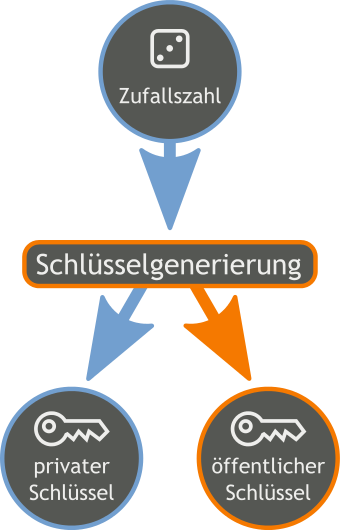
\includegraphics[scale=0.5]{Orange_blue_public_private_keygeneration} \\
\caption{Schlüsselgenerierung (aus \cite{wikipedia_keygen})}
\label{fig:figure1}
\end{figure}

Jetzt hat man den Verschlüsselungsschlüssel $(e, n)$ und den Entschlüsselungsschlüssel $(d, n)$. \\
$p$, $q$ und $\phi(n)$ sollten geheim gehalten bzw vernichtet werden, da diese Rückschlüsse auf $d$ möglich machen. Der Prozess wird in Abbildung \ref{fig:figure1} dargestellt (Alice und Bob sind in der Kryptograhie übliche Namen). Nun ist es möglich Texte zu ver- und entschlüsseln. 

Als Beispiel wählen wir $p=11$ und $q=13$.
Zuerst wird dann $n$ berechnet:
$$n = 11*13 = 143$$

Danach wird $\phi (n)$ wie folgt berechnet:
$$\phi(n) = (p-1)*(q-1) = \phi(11*13) = (11 - 1) * (13-1) = 10 * 12 = 120$$

Als letzter Schritt werden noch $e$ und $d$ berechnet, wobei für $e$ die sehr häufig verwendete Zahl 65537 gewählt wird. \cite[S.2735]{eNumber}  $d$ wird dann aus $e$ und $\phi(n)$ berechnet:
$$e * d = 1 \bmod \phi(n) = 65537 * d = 1 \bmod 120$$
$$ d = 113$$


	\subsection{Ver- und Entschlüsselung}
	Um eine Nachricht $m$ mit dem RSA-Algorithmus verschlüsseln zu können, wird der öffentliche Schlüssel $(e,n)$ benötigt.
	Als erstes muss die Nachricht in eine Zahl $m$ umgewandelt werden \footnote{Für den Umwandlungsprozess siehe \ref{chap:digital_text}} und auf eine Yahl zwischen 0 und $n-1$ bringen (Für längere Nachrichten siehe \ref{cha:hole_text}).
	Zum Verschlüsseln einer Nachricht \textit{m} werden nun der öffentliche Schlüssel ($e, n$) und $m \in \mathbb{N}$ und $m < n-1$ benötigt. (\textit{e} und \textit{n} sind hierbei positive Zahlen).\cite[6]{rsaOriginalPaper} Danach wird \textit{m} wie folgt in \textit{c} verschlüsselt \cite[S.6]{rsaOriginalPaper}: 
	$$c = m^e \bmod n$$
	Für die Entschlüsselung wird der gleiche Prozess wiederholt, nur dass dafür der private Schlüssel $(d,n)$ benötigt wird. Für \textit{m} wird diesmal \textit{c} verwendet wird und anstatt \textit{e} wird dann \textit{d} verwendet \cite[S.6]{rsaOriginalPaper}:
	$$m = c^d \bmod n$$
	
%	\begin{figure}[h!]
%	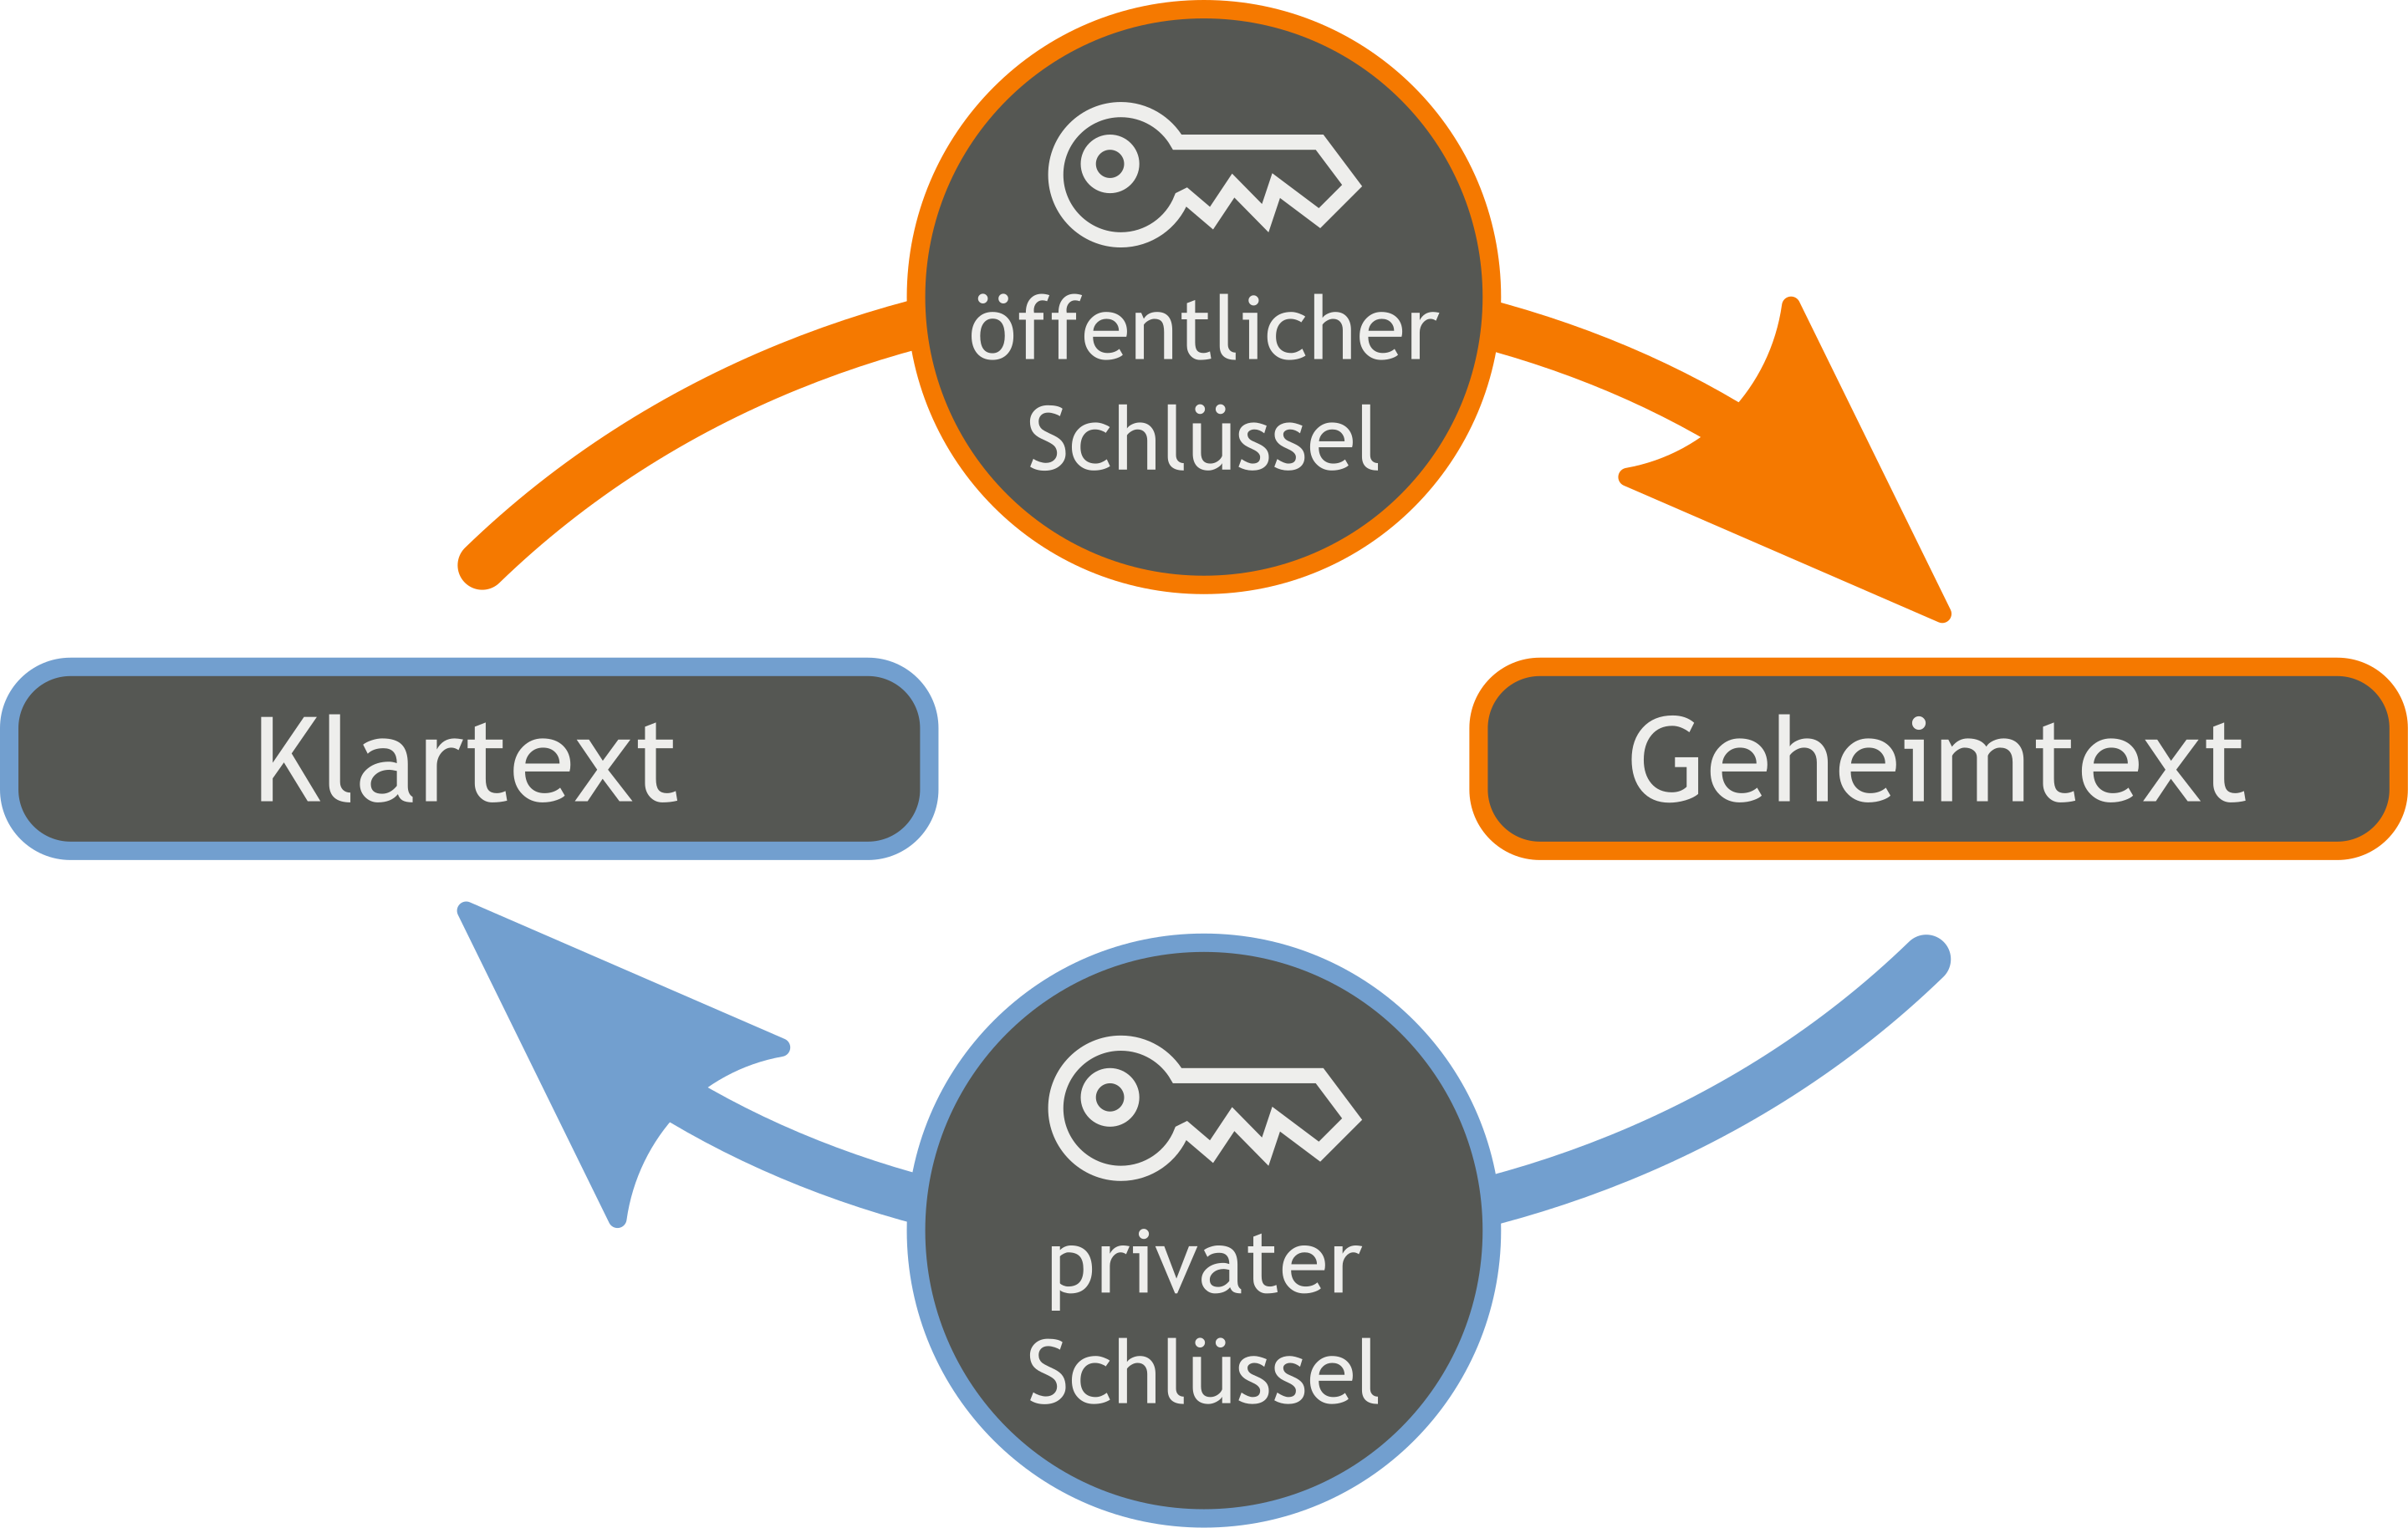
\includegraphics[scale=0.1]{Orange_blue_public_key_cryptography_de.svg.png} \\
%	\caption{Der Ver- und Entschlüsselungsprozess (aus \cite{wikipedia_enc_dec})}
%	\label{fig:figure1}
%	\end{figure}
	
	Als Beispiel verschlüsseln wir die Zahl $m = 76$. Hierbei sind $e=65537$ und $n=143$ gewählt.

	\begin{equation}
	\begin{split}
	c & = m^e \bmod n \\
	 &  = 76^{65537} \bmod 143 \\
 	& = 98
	\end{split}
	\end{equation}
	Unsere Verschlüsselte Nachricht ist nun also $c = 98$. Um daraus wieder \textit{m} zu berechen, wird mithilfe von $d$ wieder $m$ berechnet. Hierbei ist $d=113$ und wieder $n=143$ gewählt:
	\begin{equation}
	\begin{split}
	m & = c^d \bmod n \\
	 &  = 98^{113} \bmod 143 \\
 	& = 76
	\end{split}
	\end{equation}
	
	Somit ist nun eine vollständige Verschlüsselung möglich, ohne, dass sich beide Parteien kennen müssen, da jeder mithilfe des öffentlichen Schlüssels eine Nachricht verschlüsseln kann, aber nur der Besitzer des privaten Schlüssels diese Entschlüsseln kann.

	\subsection{Die Mathematik hinter dem RSA-Algorithmus}
	Um verstehen zu können, warum RSA funktioniert, muss man mathematisch die Gültigkeit der Gleichung
	\begin{equation}\label{eq:fermat}
 x = y^d \bmod n
 \end{equation}

 beweisen, sodass $c^d \bmod n$ wieder $m$ ergibt. ($x$ stellt hierbei unsere Nachricht m und y unsere verschlüsselte Nachricht c da.) Dafür wird der Satz von Euler-Fermat benötigt: \\
	Sind a und n teilerfremde Zahlen mit $1 < a < n$, so gilt
	$$a^{\phi (n)} \equiv 1 \bmod n $$
	
	Es soll im folgenden nicht dieser Satz bewiesen werden, sondern mit ihm die Gleichung (\ref{eq:fermat}), wenn $x \neq p$ und $x \neq q$ gilt, da für den Satz von Euler-Fermat $x$ und $n = p*q$ teilerfremd sein müssen. \\
	
	Es folgt die Umformung von \citeauthor{frauenhofer}:
	\begin{align*}
	 y^d \bmod n & = (x^e \bmod n)^d \bmod n & \\
	 & = (x^e)^d \bmod n &\\
 	 & =x^{ed} \bmod n &  \parbox[t]{4cm}{e ist das multiplikative Inverse zu d, also $e * d \bmod m \equiv 1$ es folgt also daraus, dass es kein $k \in \mathbb{Z}$ gibt, so dass $e*d=k*m+1$}\\
 	 & =x^{k*m+1} \bmod n & \\
 	 & =x^{k*m}*m \bmod n & \\
 	 & =((x^m)^k \bmod n) * (x \bmod n) \bmod n & \\
 	 & =(x^m \bmod n)^k * (x \bmod n) \bmod n & \\
 	 & =(1^k \bmod n) * (x \bmod n) \bmod n &  \parbox[t]{4cm}{wegen des Satzes von Euler-Fermat (sofern x und n teilerfremd sind), da $m = (p - 1)(q - 1) = \phi(n)$ gesetzt wurde} \\
 	 & = 1 * x \bmod n & \\
 	 & = x &
 	\end{align*} \cite[S.15]{frauenhofer}

	Mit dieser Umformung konnte die Gleichung (\ref{eq:fermat}) bewiesen werden 
	
	\subsection{Verschlüsselung ganzer Texte}
		\label{cha:hole_text}

	Die Schwierigkeit, ganze Texte zu verschlüsseln, liegt darin, dass die Nachricht $m$ nicht großer als $n - 1$ sein darf. Eine Möglichkeit dieses Problem zu umgehen, ist es, die Nachricht in verschiedene kleine Blöcke zu unterteilen und dann jeden Block einzeln zu verschlüsseln. Das hat aber immer noch den Nachteil, dass der RSA Algorithmus sehr langsam ist, und deshalb für eine große Nachricht $m$, auch wenn sie in kleine Blöcke unterteilt ist, sehr lange bräuchte. Eine sinnvollere, und auch weit aus verbreitete Lösung ist es mit dem RSA Algorithmus einen symmetrischen Schlüssel zu verschlüsseln. Für die genaue Funktionsweise siehe Kapitel \ref{cha:hybrid}.


\section{Mögliche Angriffspunkte}
Wie alle Arten der Verschlüsselung, weist der RSA Algorithmus mehrere potentielle Schwachpunkte auf. Er hat tendenziell auch mehr Schwachstellen, als andere Verschlüsselungsverfahren, da er deutlich mehr Stellen hat, an denen ein Angriff möglich wäre. Ein symmetrischer Verschlüsselungsalgorithmus hat nicht so viele Schwachstellen, bringt aber einge andere Nachteile mit sich.
	\subsection{Primfaktorzerlegung}
	\label{cha:primfaktorzerlegung}
	Es ist sehr schwierig eine Zahl $n$, die keine Primzahl ist, in ihre Primfaktoren zu zerlegen. Aktuell gibt es keinen Algorithmus, der dies für sehr große Zahlen bewältigen kann. Sollte es einen Algorithmus geben, der die Primfaktorzerlegung in sehr kurze Zeit bewältigen kann, würde das heißen, dass der RSA-Algorithmus nicht mehr sicher ist, da man sich dann sehr leicht $p$ und $q$ aus dem immer veröffentlichten $n$ berechnen kann und somit alle Schlüssel berechnen kann.
	
	Zum Beispiel benötigt der Quadratic Sieve Algorithmus aktuell um eine Zahl mit 512 Bits zu zerlegen aktuell bei 200.000.000 Befehle pro Sekunde in etwa 11700 Jahre. \cite[S.115]{Beutelspacher2015-jl}
	Aktuell wird ein Schlüssel mit mehr als 3000 Bits als sicher angesehen. \cite[29]{bsireco}
	 
	\subsection{Monoalphabetische Verschlüsselung}
	\label{cha:mono_enc}
	Sehr einfachen Kryptosystem, wie z.B. die Caesar-Verschlüsselung, setzen oftmals auf eine Monoalphabetische Verschlüsselung, das heißt, es wird jedem Buchstaben ein anderer Buchstabe zugeordnet. Wenn man immer einzelne Buchstaben mit dem RSA-Algorithmus verschlüsselt, hat man das Problem, das diese immer dem gleichen verschlüsselten Buchstaben zugeordnet werden. (Wie in Abbildung \ref{fig:figure4} bei A und B zu sehen). Dadurch ist die Verschlüsselung dann nicht mehr sicher und kann sehr einfach mit Hilfe von statistischen Tabellen über die Häufigkeit eines Buchstabens geknackt werden. \footnote{Mehr dazu in \cite{mono}}
	
	Um diese Schwachstelle zu beseitigen, kann man anstatt einzelne Buchstaben zu verschlüsseln, ganze Blöcke an Buchstaben verschlüsseln. Hierbei ist zu beachten, dass jeder Block, umgerechnet in eine Zahl, kleiner als \textit{n} sein muss. Jetzt ist es nicht mehr möglich Rückschlüsse auf die verwendeten Buchstaben zu machen, z.B. wurden bei den unteren beiden Beispielen in Abbildung \ref{fig:figure4} nur A an die Stelle von B und B an die Stelle von A gebracht und es kommt eine ganz andere Zahl raus.


\begin{figure}		
\includegraphics[scale=0.6]{rsa_mono} \\
\caption{Verschlüsselung verschiedener Buchstaben mithilfe des ASCII Standards und des RSA-Algorithmus}
\label{fig:figure4}
\end{figure}
	
\pagebreak

\section{Anwendungsbereiche in der IT - Sicherheit}
	\subsection{Digitale Nachrichten}
	\label{chap:digital_text}
Um eine Nachricht, hier genannt \textit{m}, mit einem Computer verarbeiten zu können, muss diese erst in Zahlen umgewandelt werden. Dafür existiert der ~ASCII~ Standard, mit dem Computer Buchstaben in Zahlen umwandeln können. Jede Nachricht \textit{m} muss kleiner sein als \textit{n}. In der Realität spielt das allerdings keine Rolle, da normalerweise Werte für \textit{n} mit mehr als 100 Stellen verwendet werden und der normale ASCII Standard 7-Bit Werte und der erweiterte ASCII Standard 8-Bit Werte verwendet \cite[S.5]{rowland}.\footnote{7-Bit hat Zahlen bis 128, 8-Bit bis 256}
	
	\subsection{Digitale Signatur}
	\label{cha:digital_signature}
	Der RSA-Algorithmus kann auch genutzt werden, um Nachrichten zu signieren. Durch das Signieren von z.B. Emails kann der Empfänger sicherstellen, dass die Nachricht von dem Besitzer des zugehörigen privaten Schlüssels verschickt wurde. Diese Funktion der Signatur wird auch genutzt, um die Fälschungssicherheit und Originalität von  Dokumenten sicherzustellen. Um bei einer Signatur nicht die Länge der Nachricht zu verdoppeln, wird diese mithilfe einer Einwegfunktion auf eine vordefinierte Länge gebracht. Denn wenn man die ganze Nachricht verschlüsseln würde, würde sich die Länge einer signierten Nachricht verdoppeln, da diese dann aus der Nachricht und der verschlüsselten Nachricht bestehen würde. \cite[S.15f]{Beutelspacher2015-jl} \footnote{Siehe Kapitel \ref{ch:einweg} auf Seite \pageref{ch:einweg}}\\

Als erstes wandelt man die Nachricht mithilfe eines Standards in Zahlen um. Mithilfe eines Hashing-Algorithmus wird nun der Hash-Wert der zu signierenden Nachricht berechnet. Dieser Wert wird dann mit dem privaten Schlüssel, dem Encryption-Key, der normalerweise der öffentliche Schlüssel ist, verschlüsselt. %Schöner formulieren
	Der Decryption-Key wird dann, anders als wenn man eine geheime Nachricht versenden will, veröffentlicht. \cite[S.15f]{Beutelspacher2015-jl}\\
	Die originale Nachricht wird dann zusammen mit der digitalen Signatur verschickt und der Empfänger entschlüsselt diese dann mithilfe des öffentlichen Schlüssels wie folgt:\\
	Als erstes generiert der Empfänger mithilfe des Hash-Algorithmus einen Hash-Wert von der Nachricht, die auf ihre Echtheit überprüft werden soll. Dann wird mit dem öffentlichen Schlüssel des Senders der, an die Nachricht angehängte, verschlüsselte Hash-Wert des Senders entschlüsselt. \\
Wenn der generierte und der entschlüsselte Hash-Wert übereinstimmen, kann sicher festgestellt werden, dass die Nachricht nicht verändert wurde. \\
Wenn eine dritte Person die Nachricht abändern würde, wäre der Hash-Wert beim Empfänger für diese Nachricht ein anderer, da der Hash-Algorithmus schon bei der Änderung eines einzelnen Bits einen anderen Hash-Wert ausgibt. Wenn dieser dann mit dem verschlüsselten Hash-Wert verglichen wird, kann festgestellt werden, ob die Nachricht im Original vorliegt, denn wenn dem nicht so ist stimmen die Hash-Werte nicht mehr überein. \cite[S.15f]{Beutelspacher2015-jl}\\


%TODO wenn noch mehr text  --> https/tls

\begin{figure}
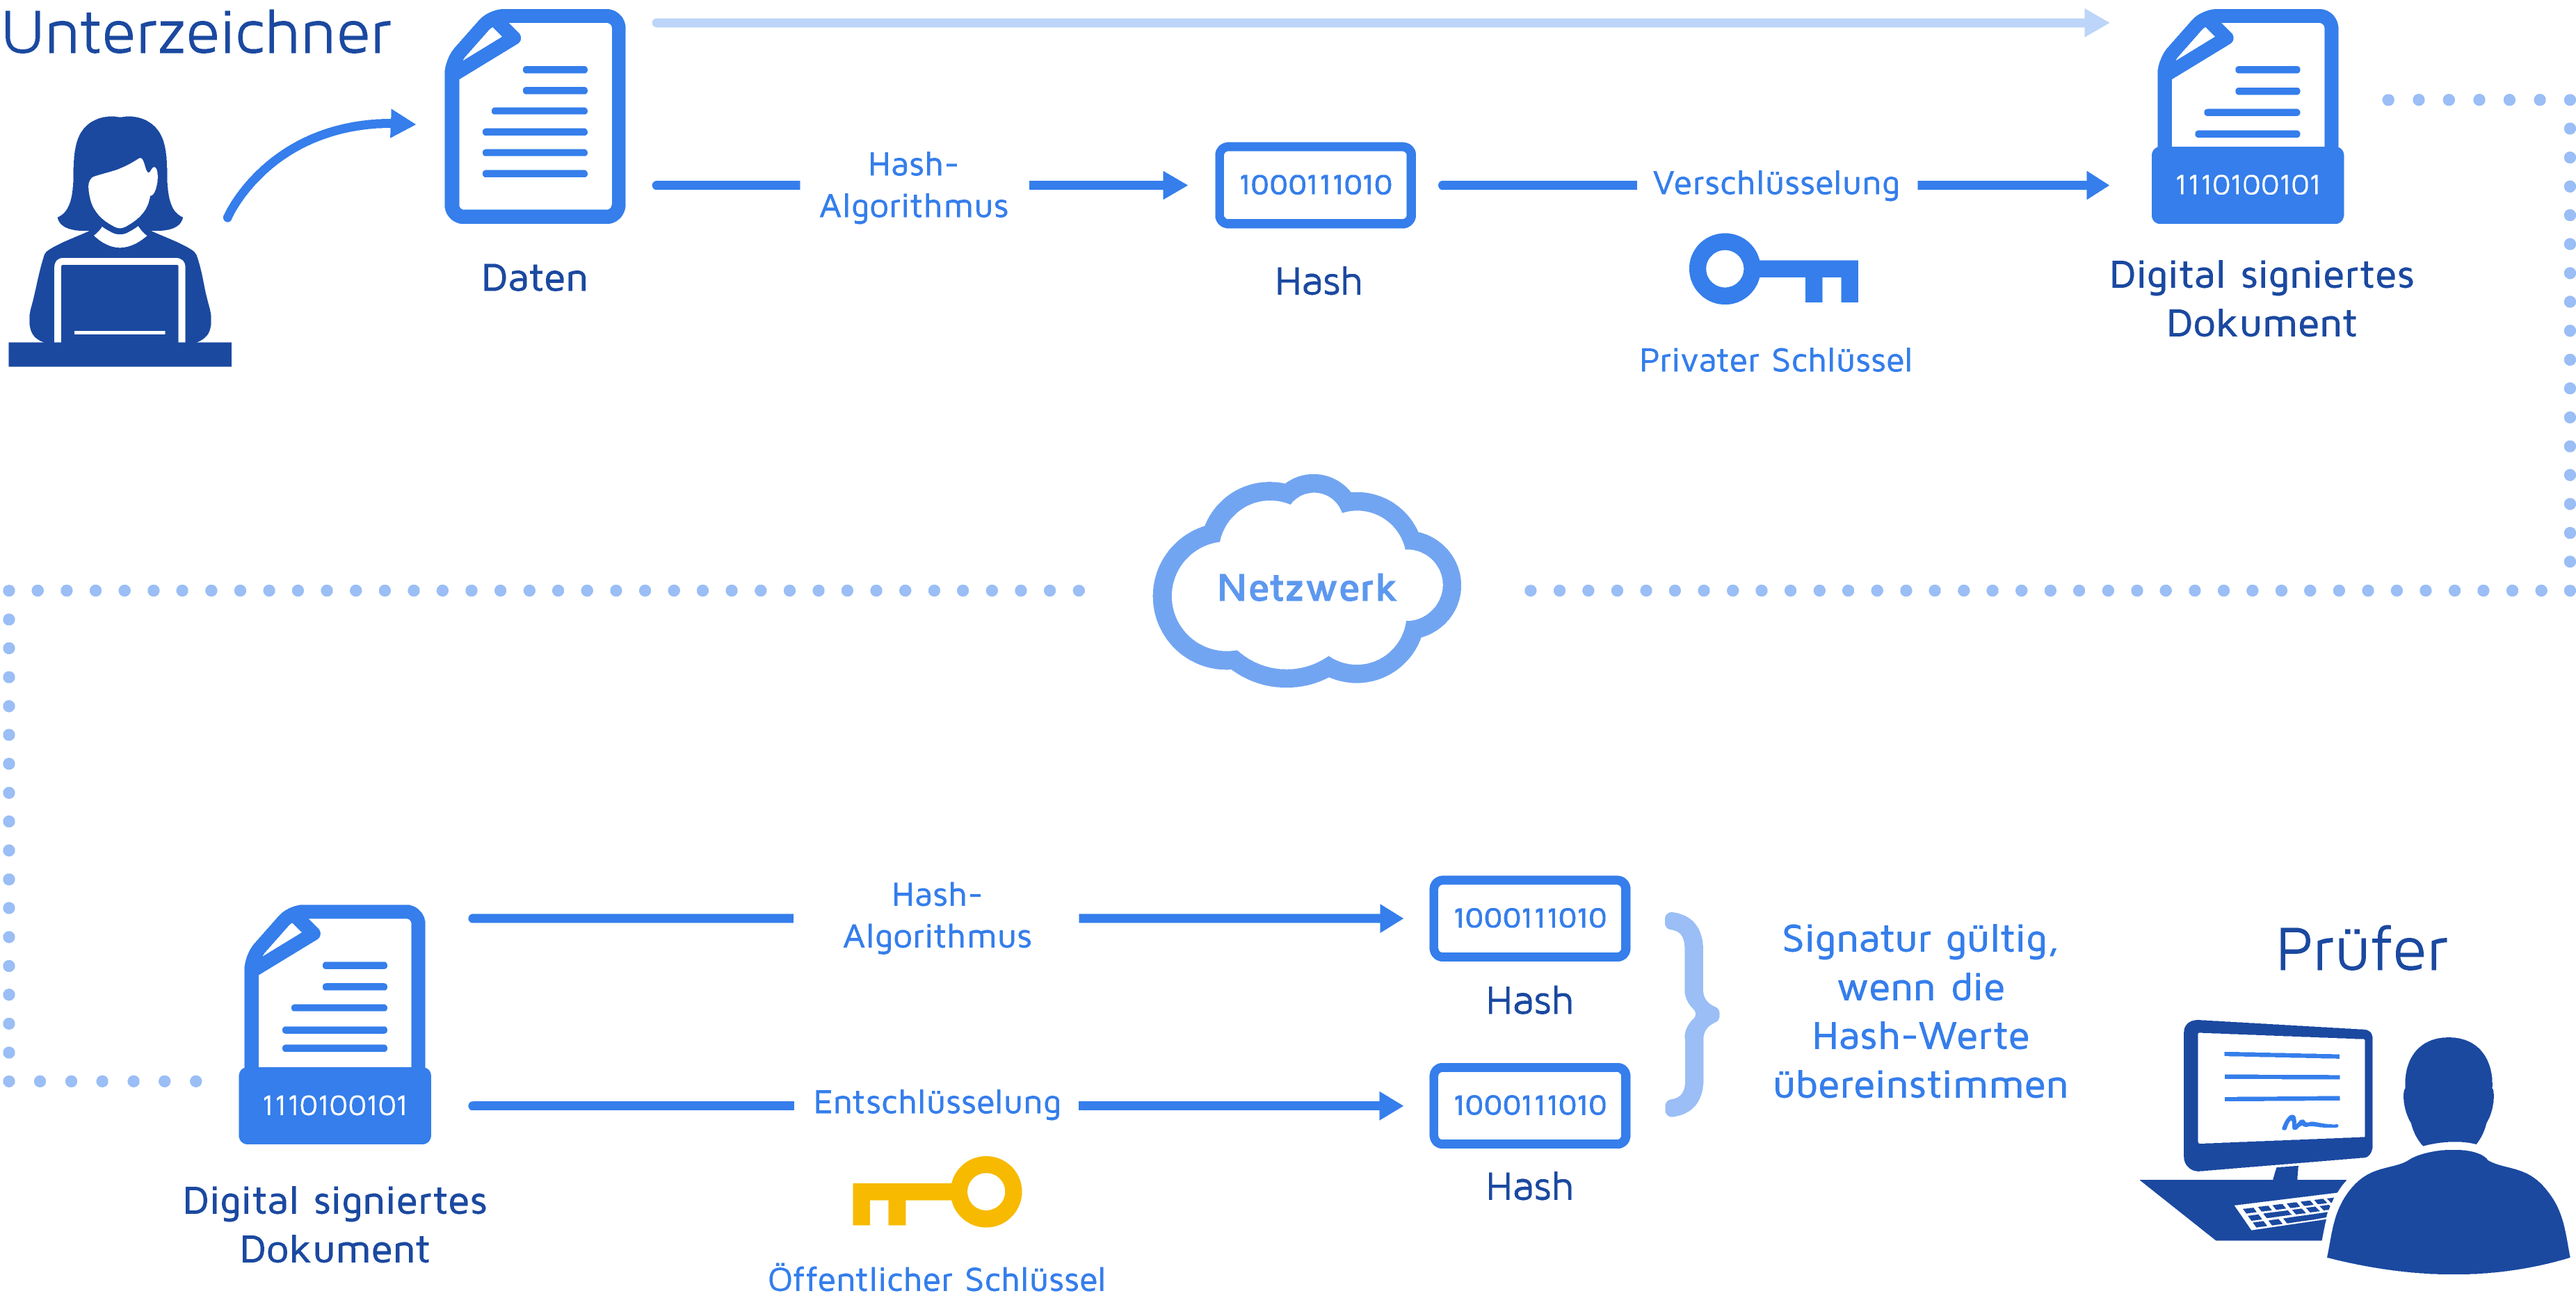
\includegraphics[scale=0.45]{Dokument_digitale_Signatur} \\
\caption{Ein Dokument digital signieren (aus \cite{digitalsignature})}
\label{fig:figure3}
\end{figure}

Das ganze funktioniert dann wie folgt nach \citeauthor{Beutelspacher2015-jl} aus \cite[S.15f]{Beutelspacher2015-jl}:

Als erstes berechnet man den Hash-Wert mithilfe einer Einwegfunktion:
$$ {h_{berechnet} = e(m)} $$

Dann vershlüsselt man mit dem RSA-Algorithmus den Hash-Wert \textit{h} und erhält die Signatur \textit{s}
$$ {s = h_{berechnet}^e \bmod n} $$

Diese Signatur wird dann an die Nachricht angehängt und anschließend veröffentlicht.
Der Empfänger kann dann mit den folgenden Schritten die Integrität der Nachricht sicherstellen:

Als erstes wird erneut h von der empfangenen Nachricht $m$ bestimmt:
$${h_{empfangen} = e(m) }$$
Dann muss die Signatur wieder entschlüsselt werden:
$$ {h_{entschluesselt} = s^d \bmod n} $$
Anschließend werden diese beiden Hashwerte verglichen und wenn diese gleich sind, kann man davon ausgehen, dass die Nachricht nicht verändert wurde. \\


Beispiel: Die digitale Signatur von \textit{m} = 8:\\ 
Angenommen:
$${ \textit{m} = 8 }$$
$${ \textit{n} = 187 }$$
$${ \textit{d} = 59 }$$
$${ \textit{e} = 19 }$$


Erst wird der Hash-Wert von \textit{m} berechnet...
$$ {16 = e(8)} $$	

...und dann mit der RSA-Funktion verschlüsselt: %richtige Formulierung?
$$ {152 = 16^{19} \bmod 187} $$	

Um jetzt sicherzustellen, dass die Nachricht nicht verändert wurde, wird erneut der Hash Wert berechnet:
$$ {16 = e(8)} $$	
und dann die Signatur $s$ entschlüsselt:
$$ {16 = 152^59 \bmod 187} $$

Werden nun beide Ergebnisse verglichen, so wird ersichtlich, dass die Nachricht nicht verändert wurde

	 	
	\subsection{Hybride Verschlüsselung}
		\label{cha:hybrid}
		
		
		Wenn man große Texte bzw. Dateien verschlüsseln möchte, brauchen verschieden Algorithmen unterschiedlich lange. Bei der Verschlüsselung mit dem RSA-Algorithmus entsteht das Problem, dass dieser für immer größer  werdende Texte immer länger braucht, wie in Abbildung \ref{fig:figure5} zu sehen ist.

\begin{figure}[h]		
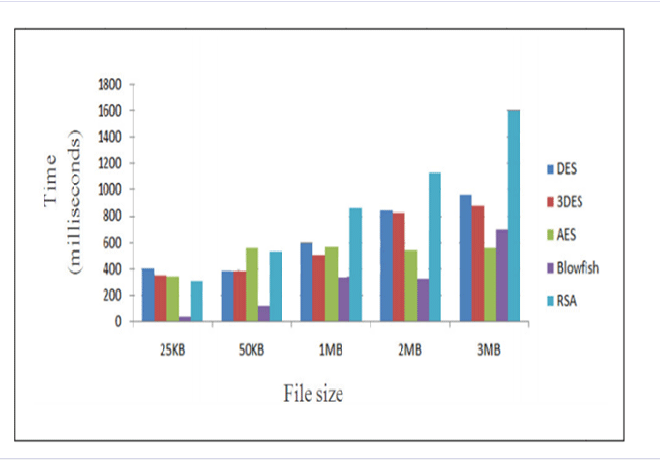
\includegraphics[scale=0.6]{rsa_time} \\
\caption{Decryption time vs. File size for DES, 3DES, AES, Blowfish and RSA (aus \cite{rsatime})}
\label{fig:figure5}
\end{figure}


		Hierfür kann dann das Konzept der hybriden Verschlüsselung genutzt werden. Dabei kombiniert man eine asymmetrisches und eines symmetrisches Verschlüsselungsverfahren. Dadurch ist es möglich, die Vorteile beider Verfahren zu kombinieren. Allerdings entstehen durch die hybride Verschlüsselung einige Nachteile beispielsweise muss man dafür beide Verfahren implementieren und die Sicherheit der hybriden Verschlüsselung ist jetzt abhängig von zwei verschiedenen Verschlüsselungsalgorithmen. Das heißt, wenn eines der Verfahren nicht mehr als sicher angesehen wird, es möglich ist, die Verschlüsselung zu durchbrechen, da entweder die symmetrische Verschlüsselung nicht mehr sicher ist oder der symmetrische Schlüssel aus dem asymmetrischen Verfahren extrahiert werden kann. \cite[S.18f]{schwenk2010sicherheit}\\
		Um nun eine Nachricht verschlüsselt versenden zu können, ohne lange auf die Verschlüsselung warten zu müssen, wird als erstes ein symmetrischer Schlüssel zufällig generiert. Mit diesem wird dann die Nachricht verschlüsselt. Dann wird der asymmetrisch verschlüsselte symmetrische Schlüssel zusammen mit der verschlüsselten Nachricht versendet. \cite[S.18f]{schwenk2010sicherheit}

\pagebreak

\section{Fazit und Ausblick}
Der RSA-Algorithmus ist zweifellos eine der bedeutendsten Entwicklungen in der modernen Kryptographie und spielt eine entscheidende Rolle in der IT-Sicherheit. Er wurde 1977 von Ron Rivest, Adi Shamir und Leonard Adleman entwickelt und hat sich seither als eine der sichersten Methoden zur Verschlüsselung von Daten etabliert. Die Sicherheit des RSA-Algorithmus liegt darin, dass es nicht möglich ist eine Zahl in einer angemessenen Zeit in ihre Primfaktoren zu zerlegen. Ein Schlüsselpaar besteht immer aus zwei Teilen, ein Teil ist der dem encryption Teil $e$ beim öffentlichen und der decryption Teil $d$ beim privaten Schlüssel. Der andere Teil besteht aus $n$ und berechnet sich von den zufällig gewählten Primzahlen $p$ und $q$. Um ganze Texte verschlüsseln zu können, muss man diese in kleinere Teile unterteilen, da die Nachrichtenlänge nicht kleiner als $m$ sein darf. Mithilfe des RSA-Algorithmus können dann digitale Nachrichten versendet werden, ohne das sich die austauschenden Parteien im vorhinein treffen mussten. Für die Umwandlung von Text wird heutzutage meistens der ASCII Standard verwendet, welcher aus 7-Bit Werten besteht. Ein weiterer großer Anwendungsbereich sind digitale Signaturen, wo der mit einer Einwegfunktion berechnete Hashwert verschlüsselt wird und an die Nachricht angehängt wird. Dann kann jeder mithilfe des öffentlichen Schlüssels des Veröffentlichers die Echtheit der Nachricht validieren. Und auch sehr lange Texte können sehr einfach mithilfe des RSA-Verfahrens und einem weiteren symmetrischen Verfahren verschlüsselt werden. Dafür muss der symmetrische Schlüssel mit dem öffentlichen Schlüssel des Empfängers verschlüsselt werden und dann wird die ganze Nachricht nur noch mit dem deutlich schnelleren symmetrischen Verfahren verschlüsselt. Allerdings gibt es heutzutage auch schon effizientere asymmetrische Verschlüsselungsverfahren, unteranderem das EdDSA-Verfahren, was auf Edwards-Kurven basiert und eine deutlich kürzere Schlüsselänge als das RSA Verfahren hat. Noch dazu ist das EdDSA-Verfahren deutlich schneller im Ver- und Entschlüsseln als der RSA-Algorithmus \cite{other_keys}. Das EdDSA Verfahren findet immer mehr Beliebtheit aufgrund seiner Vorteile, dennoch ist das RSA-Verfahren das aktuell am meisten verwendete asymmetrische Verschlüsselungsverfahren auf der Welt.


\pagebreak
\section{Anhang}

\listoffigures
\pagebreak

\nocite{*}
\printbibliography

\pagebreak

Ich erkläre hiermit, dass ich die Seminararbeit ohne fremde Hilfe angefertigt und nur die im Literaturverzeichnis angeführten Quellen und Hilfsmittel benützt habe.\\
\\
\underline{Neubiberg}, den \underline{6.11.2023} \\
Ort  \hspace{2cm} Datum \\

\underline{\hspace{10cm}} \\
Unterschrift des Verfassers






\end{document}
